\documentclass[conference]{IEEEtran}

\usepackage[utf8]{inputenc}
\usepackage[T1]{fontenc}
\usepackage[english]{babel}
\usepackage{cite}
\usepackage{amsmath,amssymb,amsfonts}
\usepackage{booktabs}
\usepackage{array}
\usepackage{tabularx}
\usepackage{multirow}
\usepackage{graphicx}
\usepackage[caption=false,font=footnotesize]{subfig}
\usepackage{url}
\usepackage{xcolor}
\usepackage{hyperref}
\usepackage[section]{placeins}
\usepackage{balance}

\hypersetup{
    colorlinks=true,
    linkcolor=blue!50!black,
    citecolor=blue!50!black,
    urlcolor=blue!50!black,
    pdftitle={Residual Fine-Tuning of a TD3 Myoelectric Prosthesis Controller Under Quantized Actuation Constraints},
    pdfauthor={Cesar Zapata}
}

\newcolumntype{Y}{>{\raggedright\arraybackslash}X}
\newcolumntype{L}[1]{>{\raggedright\arraybackslash}p{#1}}
\newcolumntype{C}[1]{>{\centering\arraybackslash}p{#1}}

\title{Residual Fine-Tuning of a TD3 Myoelectric Prosthesis Controller\\Under Quantized Actuation Constraints}

\author{
\IEEEauthorblockN{C\'esar Zapata}
\IEEEauthorblockA{Research Laboratory in Artificial Intelligence and Computer Vision ``Alan Turing''\\
Escuela Polit\'ecnica Nacional\\
Quito, Ecuador}
}

\begin{document}
\maketitle

\begin{abstract}
This paper documents the full stabilization of a TD3 controller for a four-motor myoelectric prosthesis under quantized actuation. A repository audit first exposed three blocking issues that invalidated earlier headline results: an opaque legacy reward, a temporal inconsistency in the environment step, and a simulator bug that prevented meaningful motion. After correcting those issues, the project converged to a valid post-fix benchmark, \texttt{Agent7250}, trained with a 52-dimensional Markovian observation and a tracking-centered reward. Several low-risk interventions were then explored; only residual fine-tuning over the frozen benchmark produced a stronger single-run trade-off. The best such run, \texttt{Agent1850} with $\alpha_{\mathrm{res}}=0.20$, reduced action energy and saturation while preserving benchmark-level tracking. To evaluate reproducibility, this paper adds a five-seed residual campaign with seeds $\{11,22,33,44,55\}$. The aggregated result was \texttt{trackingMSE = 0.043785 $\pm$ 0.001517}, \texttt{actionL2 = 0.581119 $\pm$ 0.069363}, \texttt{saturationFraction = 0.336202 $\pm$ 0.147114}, and \texttt{deltaActionL2 = 0.344544 $\pm$ 0.036101}, with one accepted seed and four rejected runs. The revised evidence therefore supports residual fine-tuning as the most promising intervention in the repository, but not yet as a robust replacement for the benchmark. The main contribution of this paper is a reproducible, reviewer-facing account of how the benchmark was validated, why most post-benchmark interventions failed, and how repeated-run variability changes the interpretation of the residual result.
\end{abstract}

\begin{IEEEkeywords}
Myoelectric prosthesis, reinforcement learning, TD3, residual policy learning, EMG control, quantized actuation.
\end{IEEEkeywords}

\section{Introduction}
Continuous myoelectric control remains challenging because a prosthetic controller must jointly satisfy at least three constraints: accurate trajectory tracking, bounded control effort, and smooth actuator behavior. These tensions are well known in prosthetic-hand control and broader robotic manipulation literature \cite{chen2023review,done2025prostheticrl}. TD3 is an appropriate starting point because it explicitly targets continuous action spaces and mitigates function-approximation bias in actor-critic training \cite{fujimoto2018td3}.

The project lineage also benefited from an earlier internal technical manuscript on continuous TD3 prosthesis control, but that document is not used here as a citable benchmark. Instead, this paper focuses on the reproducible state of the current repository and on the institutional dataset lineage documented in the EPN thesis by Araque Guasgua \cite{araque2024thesis}. In practice, the main research question became not only whether TD3 could learn the task, but under which implementation constraints a benchmark could be considered valid, reproducible, and useful as an operational reference.

This paper makes four concrete contributions:
\begin{enumerate}
    \item it documents the technical corrections needed before a valid benchmark existed;
    \item it formalizes the final post-fix benchmark built around a tracking-centered reward and quantized effective actuation;
    \item it summarizes the main post-benchmark intervention families and explains why most of them failed;
    \item it presents residual fine-tuning over the frozen benchmark as the only intervention that improved the tracking--aggressiveness compromise in a defensible way, together with a repository-backed multi-seed reproducibility protocol for the residual method.
\end{enumerate}

\section{Related Work}
Three lines of prior work are directly relevant to this study.

First, myoelectric prosthesis control remains a broad research area where classical signal-processing pipelines, regression models, and modern learning-based controllers coexist. Chen \emph{et al.} review this landscape and emphasize the practical difficulty of balancing dexterity, robustness, and user adaptation in prosthetic hand manipulation \cite{chen2023review}. Zaim \emph{et al.} further survey machine-learning and deep-learning approaches for EMG and EEG driven upper-limb rehabilitation, highlighting reproducibility, signal variability, and transfer-to-practice as persistent challenges \cite{zaim2025systematic}. More recent reinforcement-learning examples, such as the Unity ML-Agents study by Done \emph{et al.}, reinforce that RL is a plausible tool for prosthetic control, but also highlight the gap between virtual performance and hardware deployment \cite{done2025prostheticrl}.

Second, the residual-policy literature provides a direct conceptual template for this project. Residual Policy Learning proposes freezing a useful controller and learning only a corrective term \cite{silver2018residual}. Residual formulations were later extended to shared-autonomy settings \cite{schaff2020shared} and more recent off-policy fine-tuning pipelines such as ResFiT \cite{resfit2025}. This family of methods is especially relevant here because the project already had a strong benchmark policy and the main challenge was to reduce aggressiveness without destroying its tracking behavior.

Third, constrained action interfaces matter in continuous-control RL. In this repository, the policy outputs continuous commands, but the simulator applies a threshold and a quantized PWM map before the plant sees the action. This creates a mismatch between continuous optimization and effective actuation. Related work on reward shaping and action smoothness in robotic control helps motivate why these interface details can dominate observed behavior even when the base RL algorithm is unchanged \cite{deng2025reward,lee2024smoothness}.

\begin{table}[t]
\centering
\caption{Positioning this work relative to nearby literature}
\label{tab:related-positioning}
\footnotesize
\begin{tabularx}{\columnwidth}{L{1.55cm}L{1.25cm}L{1.4cm}Y Y}
\toprule
Work & Domain & Platform & Reported emphasis & Direct comparability \\
\midrule
Chen \emph{et al.} \cite{chen2023review} & Myoelectric prostheses & Review & Broad survey of control paradigms & Conceptual only \\
Zaim \emph{et al.} \cite{zaim2025systematic} & EMG/EEG upper-limb control & Review & Reproducibility and signal-variability challenges & Conceptual only \\
Done \emph{et al.} \cite{done2025prostheticrl} & Prosthetic hand RL & Simulation & RL-driven virtual actuation & Partial: different simulator and metrics \\
Araque \cite{araque2024thesis} & Prosthesis control lineage & Simulation + hardware tests & Dataset lineage and DQN-based prototype study & Partial: data lineage, not same controller or metrics \\
This work & Four-motor prosthesis control & Simulation & Quantized effective actuation, residual TD3, benchmark trade-off & Primary result \\
\bottomrule
\end{tabularx}
\end{table}

\section{Dataset and Experimental Protocol}
All experiments in this repository use prerecorded EMG and glove trajectories stored locally under the repository folder named \texttt{Denis Dataset}. This dataset lineage is documented in the EPN thesis by Araque Guasgua \cite{araque2024thesis}. In the current repository version, the folder contains 12 dataset files corresponding to 12 participants or recording sources: \texttt{BLANCA}, \texttt{CECILIA}, \texttt{DENIS}, \texttt{EMILIA}, \texttt{GABI}, \texttt{GABRIEL}, \texttt{IVANNA}, \texttt{JOE}, \texttt{JONATHAN}, \texttt{KHAROL}, \texttt{MATEO}, and \texttt{SANDRA}. Each dataset file stores EMG repetitions, glove trajectories, and metadata. At the raw level, each EMG sample is an $m \times 8$ matrix, where the eight columns correspond to the available EMG channels.

Feature extraction converts each EMG block into 40 EMG features using five descriptors per channel: standard deviation, integral absolute envelope, mean absolute value, EMG energy, and root mean square. These five descriptors across eight channels yield the 40-dimensional EMG block, which is then embedded in the final operational observation
\begin{equation}
\texttt{markov52} = 40 + 4 + 4 + 4,
\end{equation}
where the additional terms correspond to normalized encoder positions, encoder increments, and the previous effective action. Episodes use prerecorded EMG and glove data with a maximum duration of 5~s and a control sample period of 0.2~s.

The experimental protocol is intentionally simple and should be read as such. Training and evaluation episodes are sampled from the pooled prerecorded dataset. During reset, repetitions are shuffled using MATLAB's \texttt{randperm}, and episodes alternate opening and closing trajectories. This protocol is useful for simulation-based controller development, but it is \emph{not} a subject-held-out generalization study. The present paper therefore makes no claim of inter-subject generalization, clinical transfer, or online adaptation to a live user.

\section{System Formulation}
\subsection{Observation and Control Variables}
The task consists of controlling four prosthetic motors from prerecorded EMG and glove data in simulation. The final operational observation is the \texttt{markov52} state:
\begin{equation}
s_t =
\begin{bmatrix}
\phi_t \\
\mathrm{enc}_t \\
\Delta \mathrm{enc}_t \\
\tilde{a}_{t-1}
\end{bmatrix}
\in \mathbb{R}^{52},
\end{equation}
where $\phi_t \in \mathbb{R}^{40}$ are EMG features, $\mathrm{enc}_t \in \mathbb{R}^{4}$ is the normalized encoder vector, $\Delta \mathrm{enc}_t \in \mathbb{R}^{4}$ is the encoder increment, and $\tilde{a}_{t-1} \in \mathbb{R}^{4}$ is the previously applied effective action. Compared with the earlier project-state observation design, this state preserves the EMG core while adding Markovian actuator information that proved useful after the simulator fix.

The policy outputs a continuous action
\begin{equation}
a_t \in [-1,1]^4,
\end{equation}
but the simulator applies a quantized effective command. With maximum PWM $P_{\max}=255$, activation threshold $\tau = 0.05$, and actuator levels
\begin{equation}
\mathcal{L} = \{0,64,96,128,160,192,224,255\},
\end{equation}
the implemented mapping is
\begin{equation}
\tilde{a}_{t,i} =
\begin{cases}
0, & |a_{t,i}| < \tau,\\[4pt]
\mathrm{sign}(a_{t,i}) \, \dfrac{\ell^\star}{P_{\max}}, & \text{otherwise},
\end{cases}
\end{equation}
where
\begin{equation}
\ell^\star = \arg \min_{\ell \in \mathcal{L}\setminus\{0\}} \left| |a_{t,i}| P_{\max} - \ell \right|.
\end{equation}
This quantized effective action was critical for making both the reward and the evaluation metrics physically meaningful.

\subsection{Reward}
The final operational reward is the implemented \texttt{trackingMseActionRateReward}. For motor-wise tracking error $e_{t,i} = \hat{y}_{t,i} - y_{t,i}$, action penalty weight $\lambda_a = 0.01$, and action-rate penalty weight $\lambda_{\Delta a} = 0.05$, the reward is
\begin{equation}
r_t = -\frac{1}{4}\sum_{i=1}^{4}
\left(
e_{t,i}^{2}
+ \lambda_a \tilde{a}_{t,i}^{2}
+ \lambda_{\Delta a} (\tilde{a}_{t,i} - \tilde{a}_{t-1,i})^{2}
\right).
\label{eq:reward}
\end{equation}
This formulation intentionally prioritizes tracking while treating effort and smoothness as regularizers rather than competing objectives. The design is aligned with reward-shaping guidance in robotic control, where interpretability and consistency with the physical objective are essential \cite{deng2025reward,lee2024smoothness}. The specific values $\lambda_a = 0.01$ and $\lambda_{\Delta a} = 0.05$ were inherited from the validated benchmark recipe and retained because later exploratory variants did not improve the global tracking--aggressiveness trade-off. They should therefore be interpreted as validated working settings rather than as exhaustively ablated optima.

\subsection{TD3 Configuration}
The controller uses TD3 with feedforward actor and critic networks. The base agent was trained with hidden width 64, actor learning rate $10^{-4}$, critic learning rate $10^{-3}$, discount factor $\gamma = 0.95$, minibatch size 64, and replay buffer length $10^5$. Simulation used prerecorded data, a sample period of 0.2~s, and up to 50 steps per episode. The implementation was built in MATLAB Reinforcement Learning Toolbox \cite{mathworks_td3_agent,mathworks_td3_options,mathworks_continuous_actor}.

The use of $\gamma = 0.95$ should be understood as part of the inherited validated benchmark configuration, not as a claim that it is universally optimal for continuous tracking. In particular, values such as $\gamma = 0.99$ remain reasonable candidates for future ablation and are not ruled out by the present study.

\section{From Historical Baseline to Valid Benchmark}
\subsection{Why Earlier Results Could Not Be Treated as Final Benchmarks}
The repository audit identified three issues that invalidated earlier headline results:
\begin{enumerate}
    \item the legacy reward mixed directional heuristics, inactivity bonuses, and tracking terms in a poorly interpretable way;
    \item the environment step had a temporal inconsistency between command application and reward/state update;
    \item the simulator relied on corrupted plant data, effectively preventing meaningful motion.
\end{enumerate}
These findings changed the interpretation of the project timeline. Earlier experiments remained useful as debugging and instrumentation stages, but they could not serve as quantitative baselines.

\subsection{Post-fix Benchmark Construction}
After the simulator fix, the project stabilized around a clean post-fix recipe: \texttt{markov52}, the reward in \eqref{eq:reward}, feedforward TD3, and quantized effective actuation. Three milestones summarize the validated baseline line:
\begin{itemize}
    \item a first valid 2000-episode post-fix baseline;
    \item a refined 8000-episode baseline, whose best checkpoint was \texttt{Agent7250};
    \item a 12000-episode extension, which did not improve the 8000-episode compromise.
\end{itemize}

\begin{table*}[t]
\centering
\caption{Historical progression from the valid benchmark to the residual reproducibility study}
\label{tab:main-results}
\footnotesize
\begin{tabular}{L{3.15cm}C{1.15cm}C{1.15cm}C{1.10cm}C{1.45cm}C{1.35cm}L{2.35cm}}
\toprule
Stage / agent & \shortstack{tracking\\MSE} & \shortstack{tracking\\MAE} & \shortstack{action\\L2} & \shortstack{saturation\\Fraction} & \shortstack{delta\\ActionL2} & Acceptance vs. \texttt{Agent7250} \\
\midrule
Valid post-fix baseline (2000 episodes) & 0.052805 & 0.179093 & 0.674957 & 0.474999 & 0.633264 & Inferior baseline \\
\texttt{Agent7250} (8000 episodes) & \textbf{0.043045} & \textbf{0.160336} & 0.596444 & 0.392086 & 0.321385 & Official benchmark \\
\texttt{Agent11900} (12000 episodes) & 0.045189 & 0.164639 & 0.649868 & 0.511786 & 0.305285 & Rejected \\
Residual best single run \texttt{Agent1850}, $\alpha_{\mathrm{res}}=0.20$ & 0.043445 & 0.163542 & \textbf{0.523597} & \textbf{0.272637} & \textbf{0.299262} & \texttt{ConditionB} \\
Residual 5-seed aggregate, $\alpha_{\mathrm{res}}=0.20$ & 0.043785 $\pm$ 0.001517 & 0.161675 $\pm$ 0.002406 & 0.581119 $\pm$ 0.069363 & 0.336202 $\pm$ 0.147114 & 0.344544 $\pm$ 0.036101 & 1 accepted, 4 rejected \\
\bottomrule
\end{tabular}
\end{table*}

Table~\ref{tab:main-results} shows why \texttt{Agent7250} became the official benchmark. The 2000-episode run was the first valid post-fix baseline, but the 8000-episode run materially improved tracking, action energy, saturation, and action-rate behavior at the same time. The 12000-episode extension did not surpass this compromise, indicating a practical plateau under the same formulation.

\begin{figure*}[t]
\centering
\subfloat[Training progress of the valid 8000-episode baseline.]{
    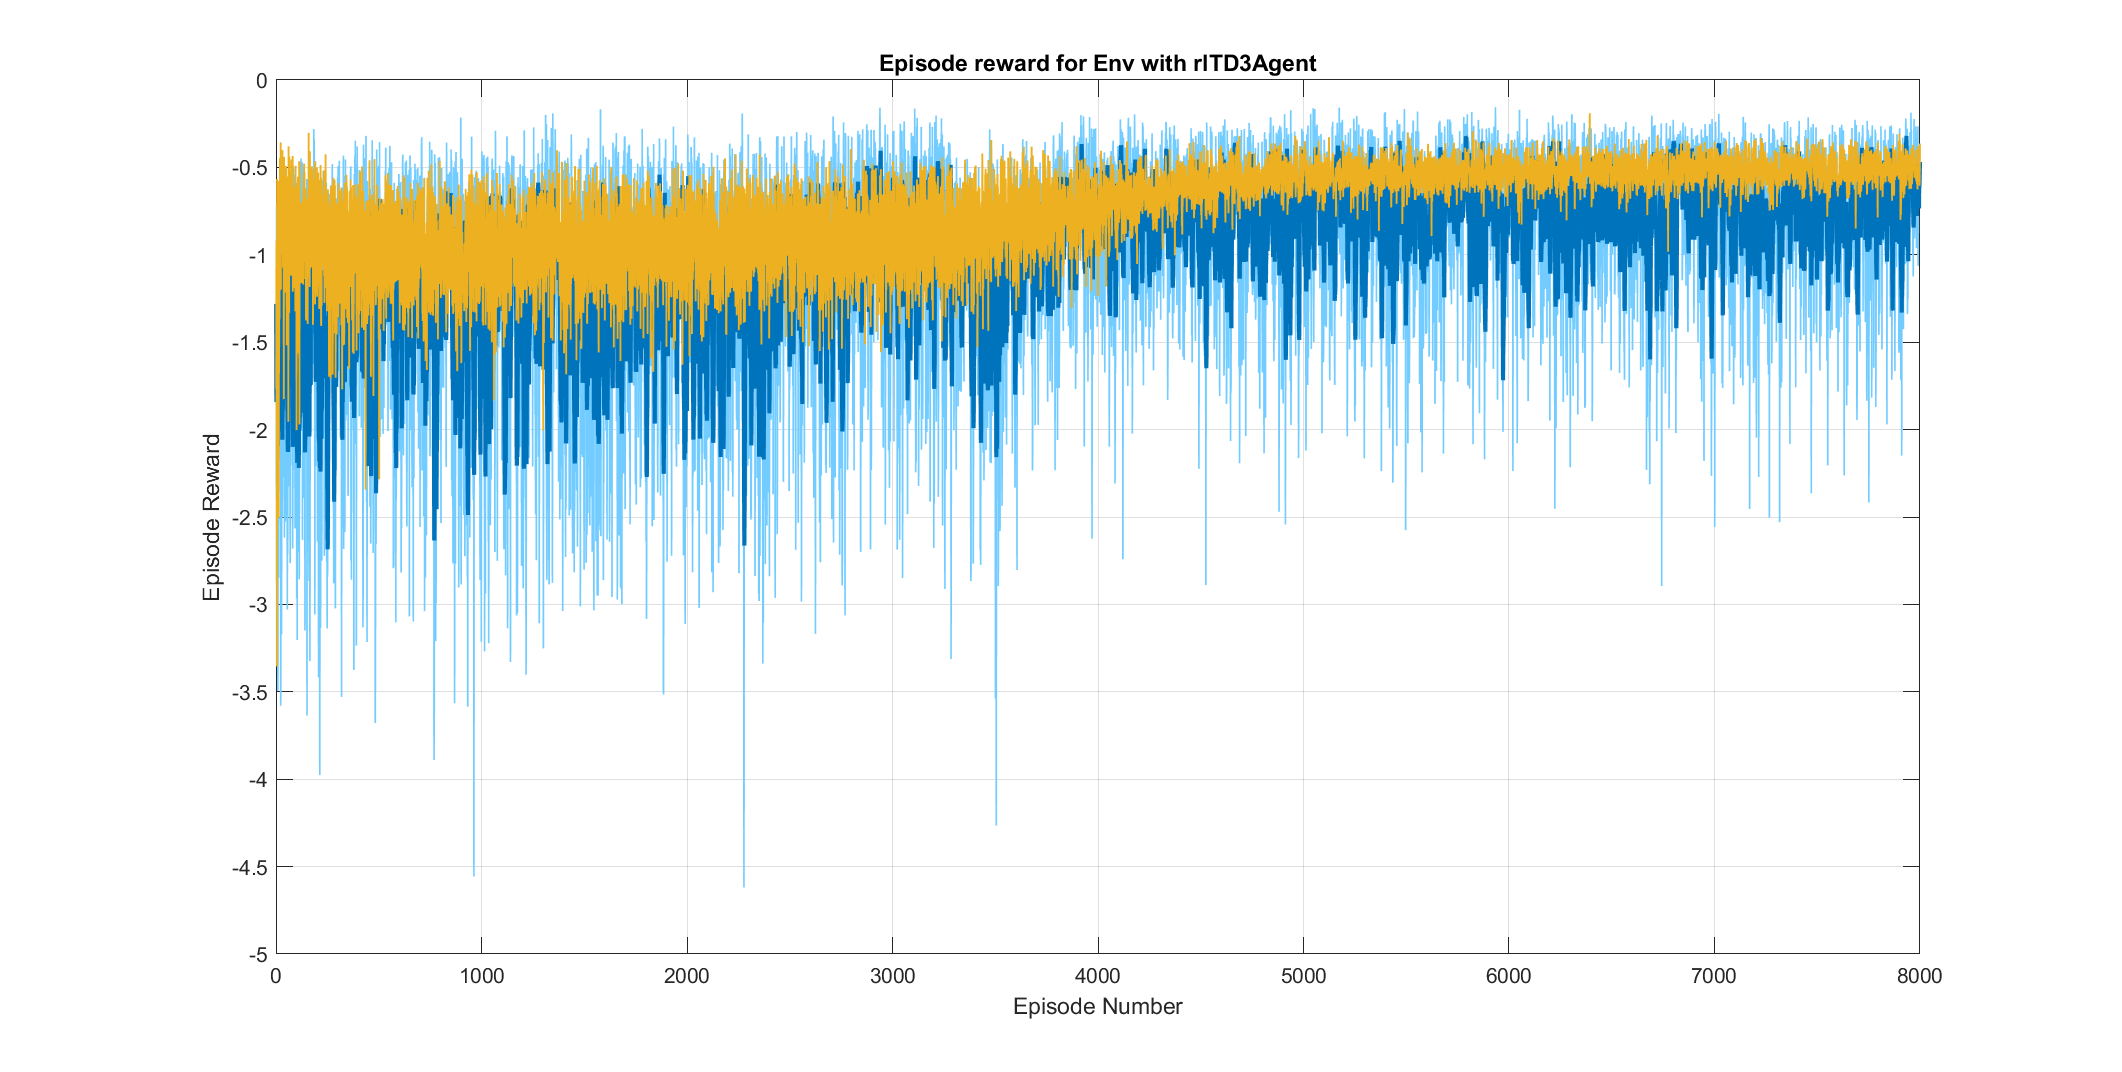
\includegraphics[width=0.49\linewidth]{figures/training_progress_8000eps_valid_baseline.png}
    \label{fig:baseline-train}
}
\hfill
\subfloat[Representative test episode for \texttt{Agent7250}.]{
    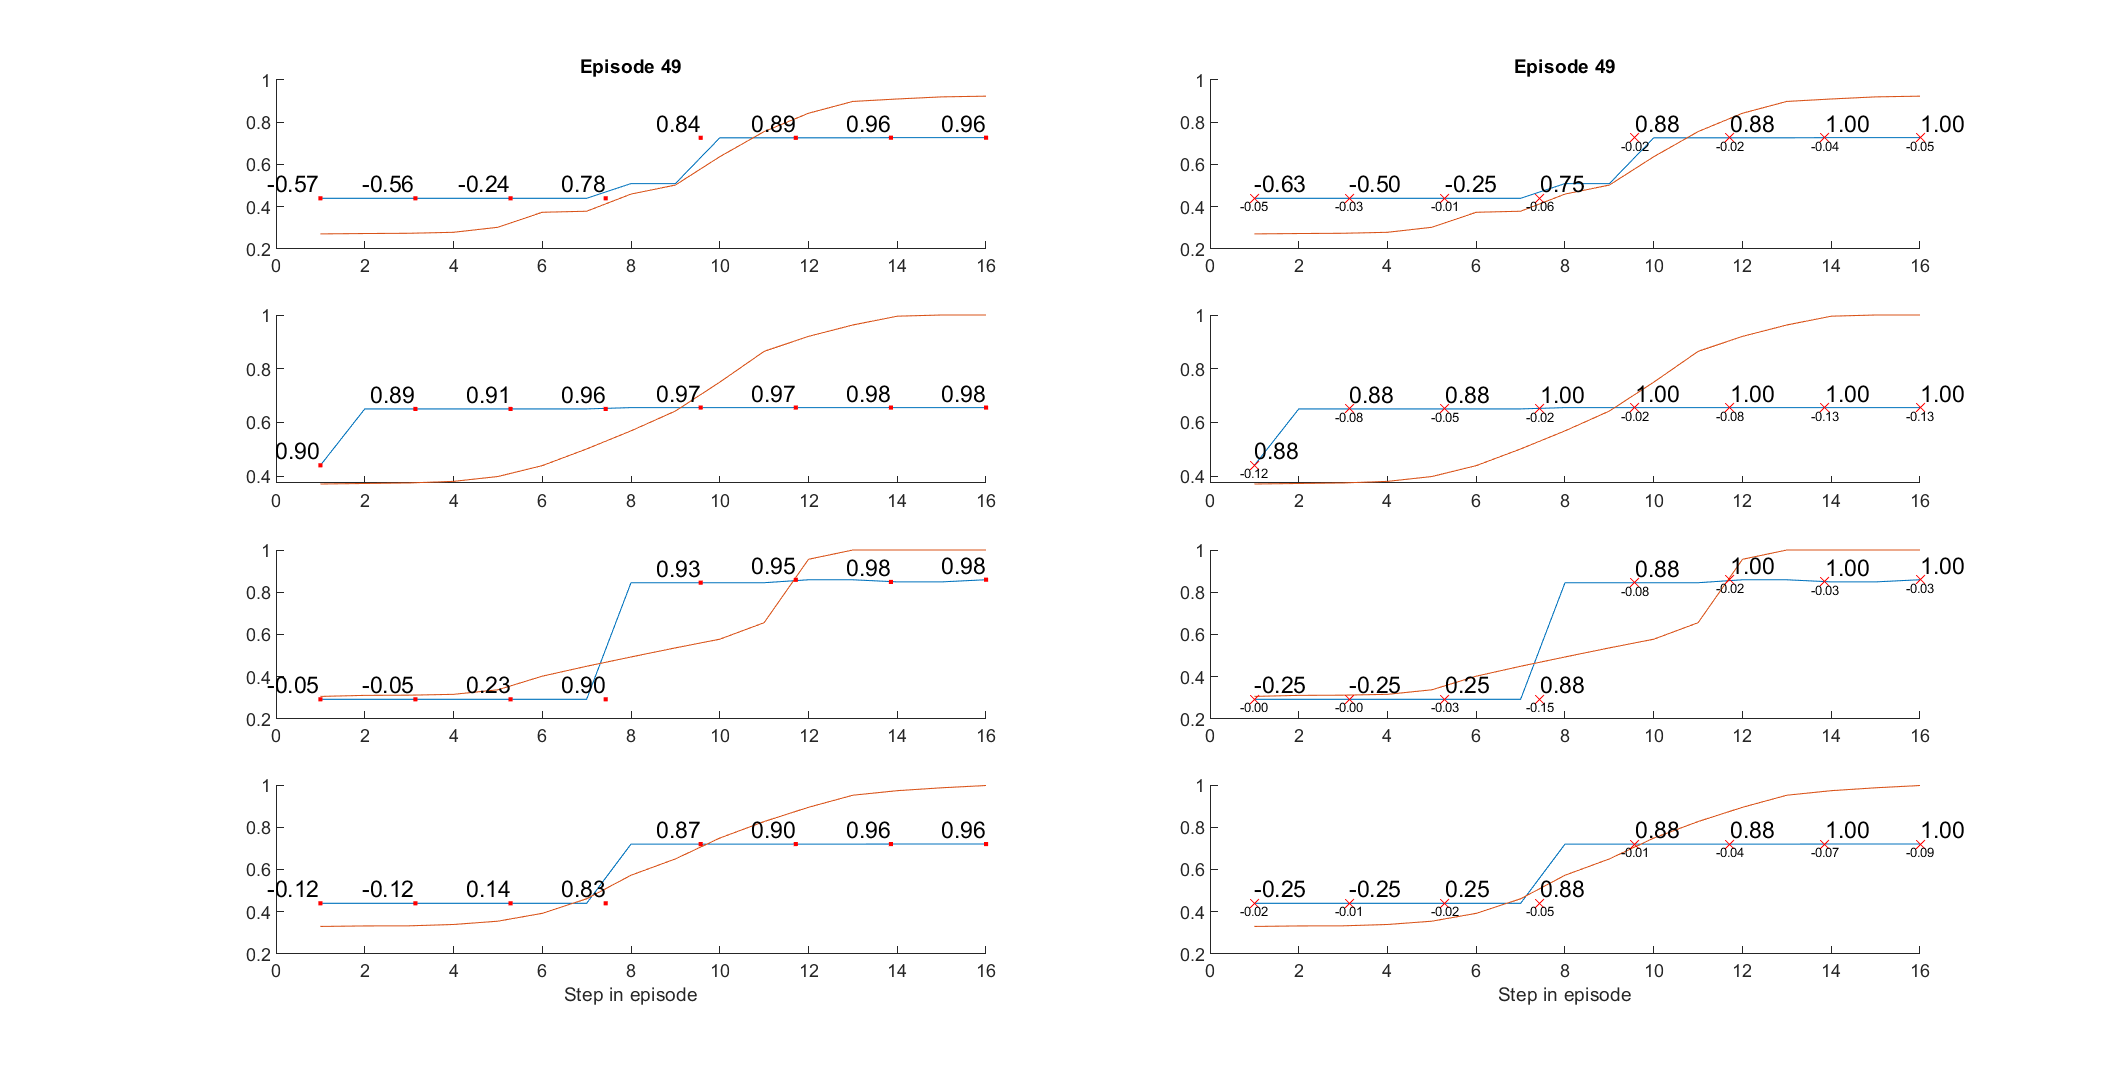
\includegraphics[width=0.49\linewidth]{figures/test_episode_49_valid_baseline_8000.png}
    \label{fig:baseline-test}
}
\caption{The validated benchmark line after the simulator fix. The late-stage improvement justified the longer 8000-episode run, and the representative test already shows good tracking with still relatively aggressive control.}
\label{fig:baseline}
\end{figure*}

\section{Why Residual Fine-Tuning Was Needed}
Once \texttt{Agent7250} was fixed as a benchmark, the main question changed. The problem was no longer ``can the controller learn tracking?'' but rather ``can we reduce aggressiveness without losing the tracking behavior already achieved?'' Several low-risk interventions were evaluated after the benchmark:
\begin{itemize}
    \item lower-exploration continuation;
    \item threshold-aware exploration;
    \item explicit saturation-penalty reward shaping;
    \item offline warm-start with behavior cloning;
    \item an aligned continuous-action warp at the actuator interface.
\end{itemize}

These experiments were informative but unsuccessful as replacements. Some made the controller too timid, while others increased edge-of-actuator usage. Fig.~\ref{fig:post7250} summarizes that phase and shows that the residual intervention was the only line that improved the global trade-off.

\begin{figure}[t]
\centering
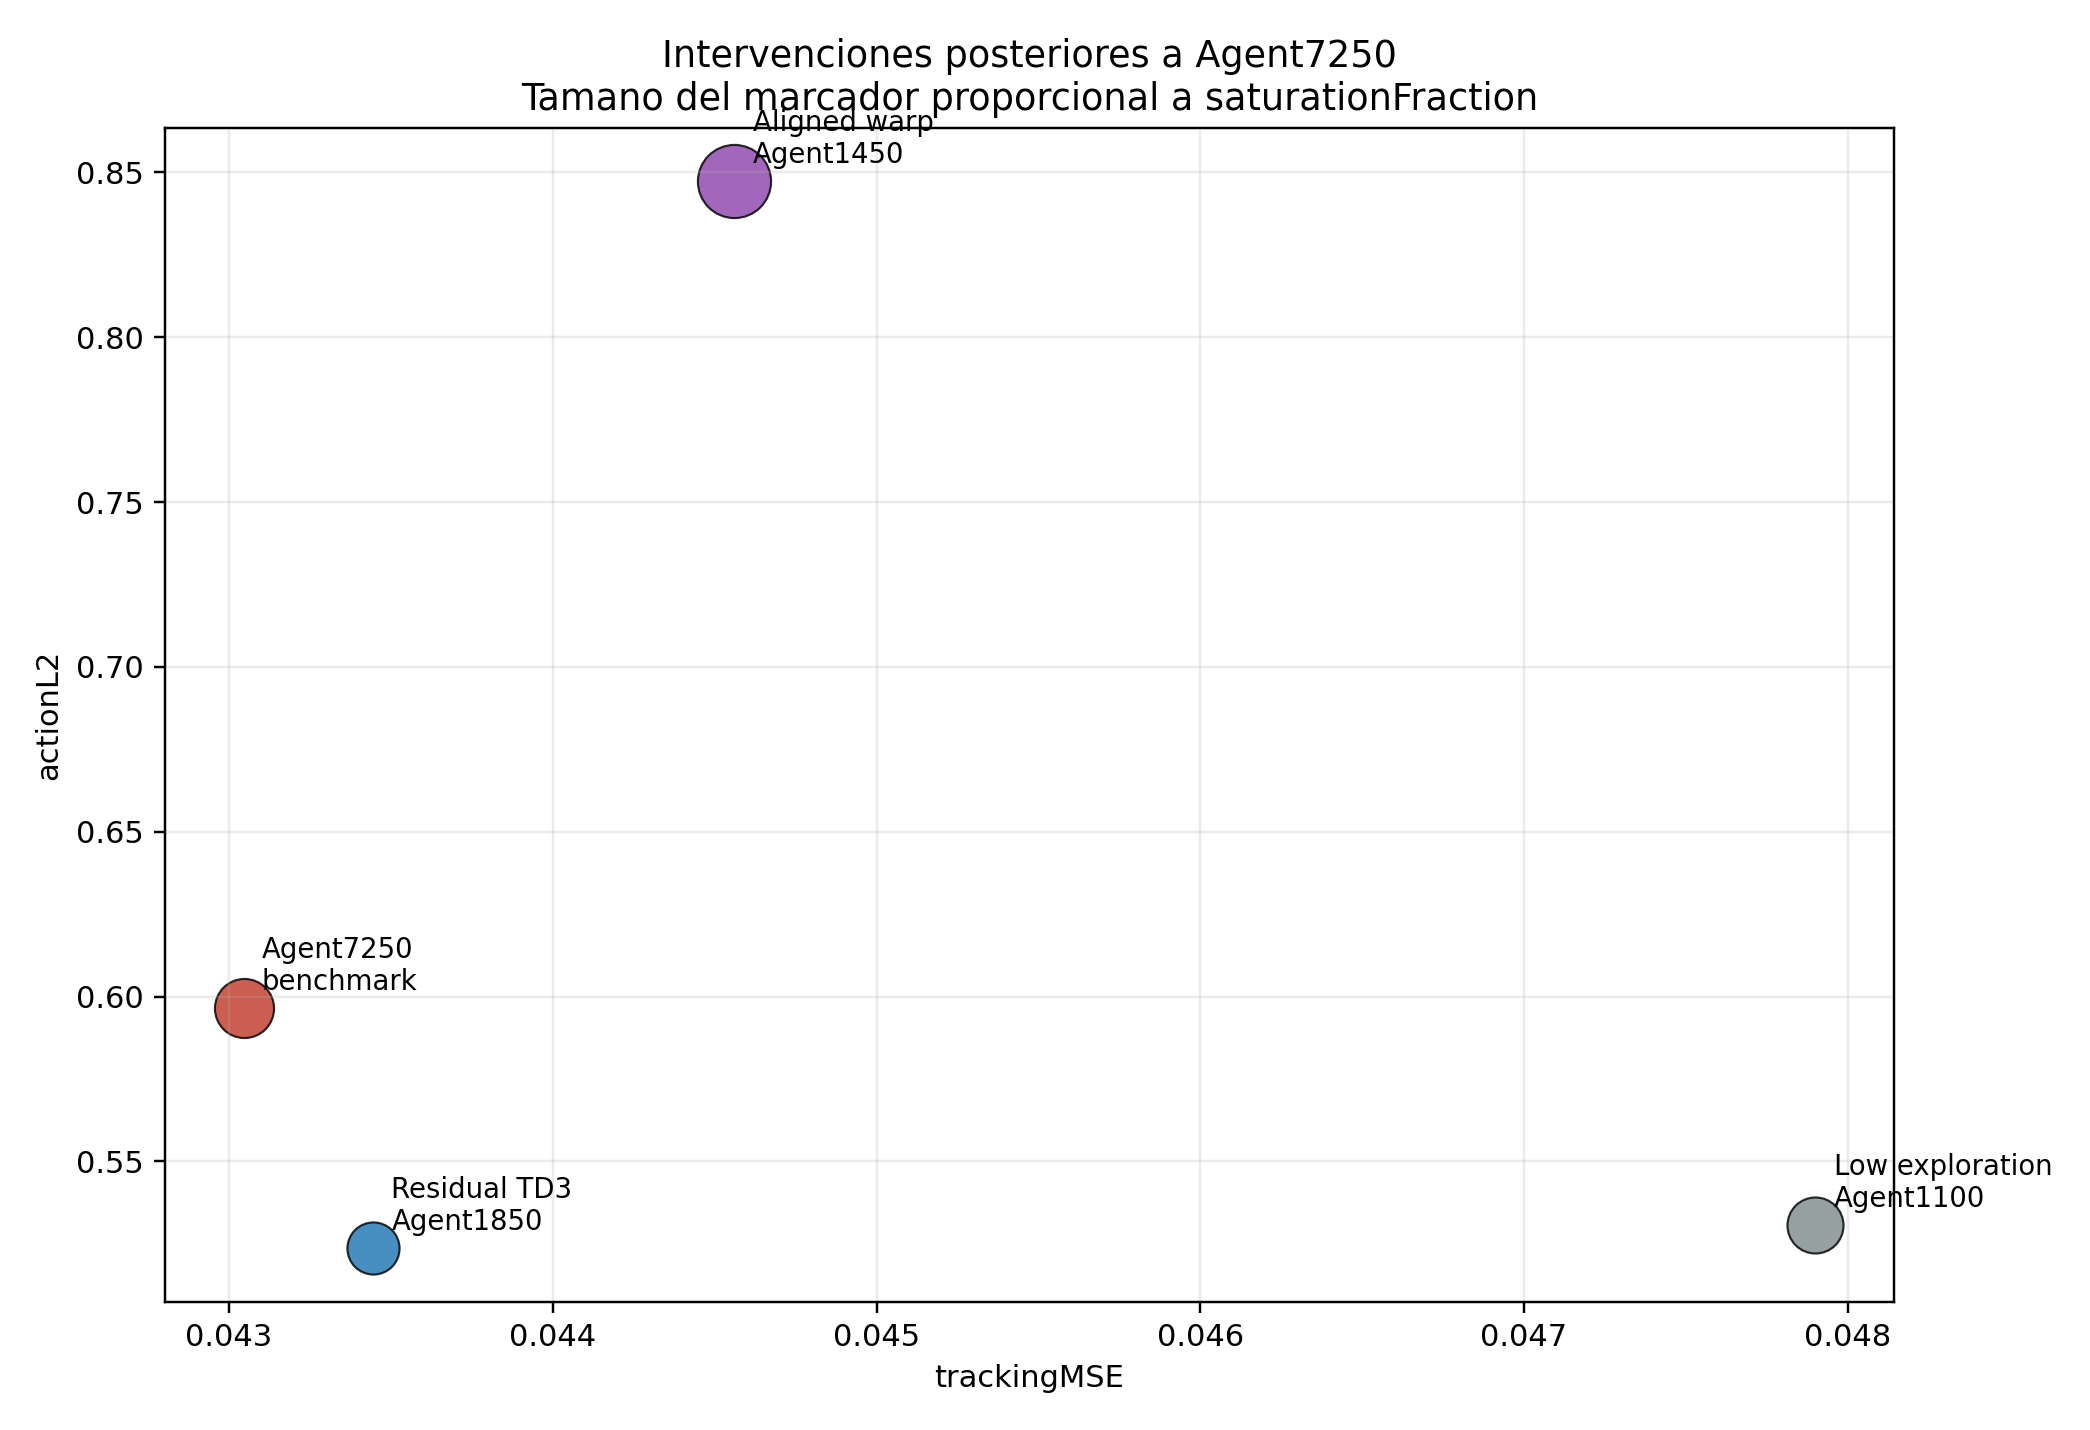
\includegraphics[width=\linewidth]{figures/post7250_interventions_tradeoff_20260326.png}
\caption{Post-\texttt{Agent7250} intervention families. Residual learning was the only line that improved the overall tracking--aggressiveness compromise instead of collapsing to a timid or overly aggressive extreme.}
\label{fig:post7250}
\end{figure}

\section{Residual Lift: Frozen-Base Residual TD3}
The final successful intervention was a residual policy built on top of the frozen benchmark. The idea follows Residual Policy Learning \cite{silver2018residual,schaff2020shared,resfit2025}: keep the base controller and learn only a bounded correction.

Let $a_{\mathrm{base}}(s)$ be the frozen action of \texttt{Agent7250}. The residual policy outputs
\begin{equation}
a(s) = \mathrm{clip}\Big(
a_{\mathrm{base}}(s) +
\alpha_{\mathrm{res}} a_{\mathrm{res}}(s, a_{\mathrm{base}}),
-1,1
\Big),
\label{eq:residual}
\end{equation}
where $a_{\mathrm{res}}$ is a learnable residual branch and $\alpha_{\mathrm{res}}$ controls how far the final policy may move away from the base action.

In the implemented actor:
\begin{itemize}
    \item the frozen base branch is copied from the benchmark actor;
    \item the residual branch receives the concatenation $[s; a_{\mathrm{base}}]$;
    \item the residual multilayer perceptron uses widths $56 \rightarrow 32 \rightarrow 32 \rightarrow 4$;
    \item the 56-dimensional input explicitly means 52 state features plus 4 base-action inputs;
    \item the critics are initialized from the base TD3 checkpoint and remain trainable.
\end{itemize}

The operator name adopted in the repository for this generic frozen-base workflow is \emph{Residual Lift}. In practice, it means that a new residual branch starts from zero while the selected base checkpoint remains frozen.

\subsection{Acceptance Rule}
All candidate policies were still judged against \texttt{Agent7250}. The strict acceptance rule required either:
\begin{itemize}
    \item \texttt{ConditionA}: better trackingMSE than the benchmark, without worsening saturation or actionL2; or
    \item \texttt{ConditionB}: trackingMSE no worse than 3\% above benchmark, at least 10\% lower saturationFraction, and at least 8\% lower actionL2.
\end{itemize}
This explicit rule prevented selection by training reward alone and kept model choice anchored to control quality rather than optimization artifacts.

\section{Residual Experiments and Reproducibility Protocol}
\subsection{Main Pilot and Follow-up Sweeps}
The main residual pilot used the frozen \texttt{Agent7250} checkpoint, residual scale $\alpha_{\mathrm{res}}=0.20$, residual hidden width 32, and low exploration noise ($\sigma = 0.02$, minimum 0.002). The best checkpoint was \texttt{Agent1850}. In the full 50-simulation visual test, it obtained the single-run values reported in Table~\ref{tab:main-results}. This was the first intervention to satisfy \texttt{ConditionB} in a single-run setting.

\begin{figure}[!t]
\centering
\subfloat[Residual pilot training progress.]{
    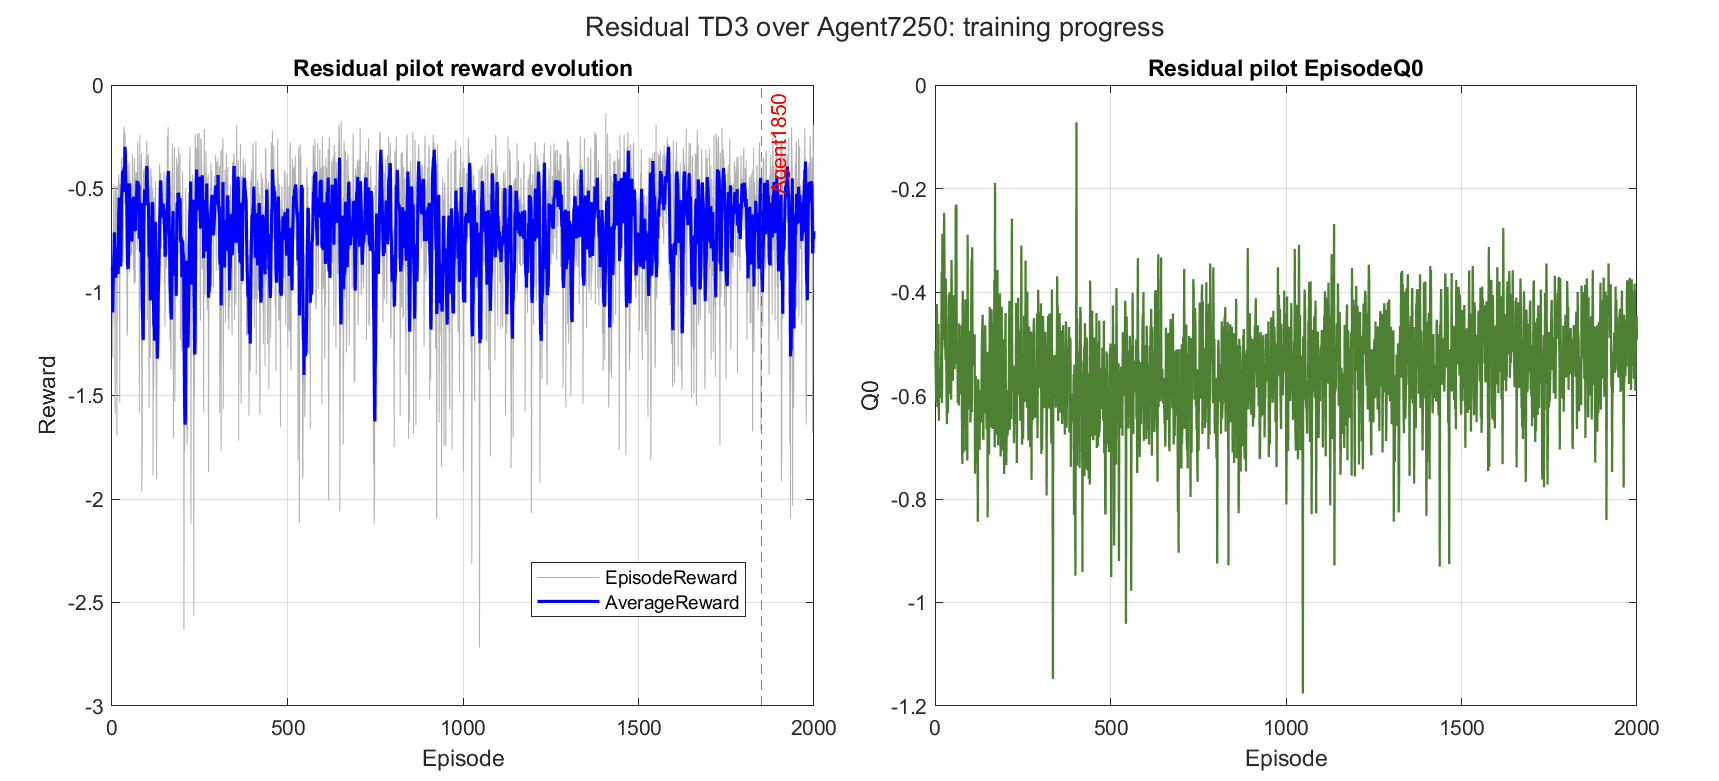
\includegraphics[width=\linewidth]{figures/residual_agent1850_training_progress_20260326.png}
    \label{fig:res-train}
}
\vspace{1mm}

\subfloat[Representative test episode for residual \texttt{Agent1850}.]{
    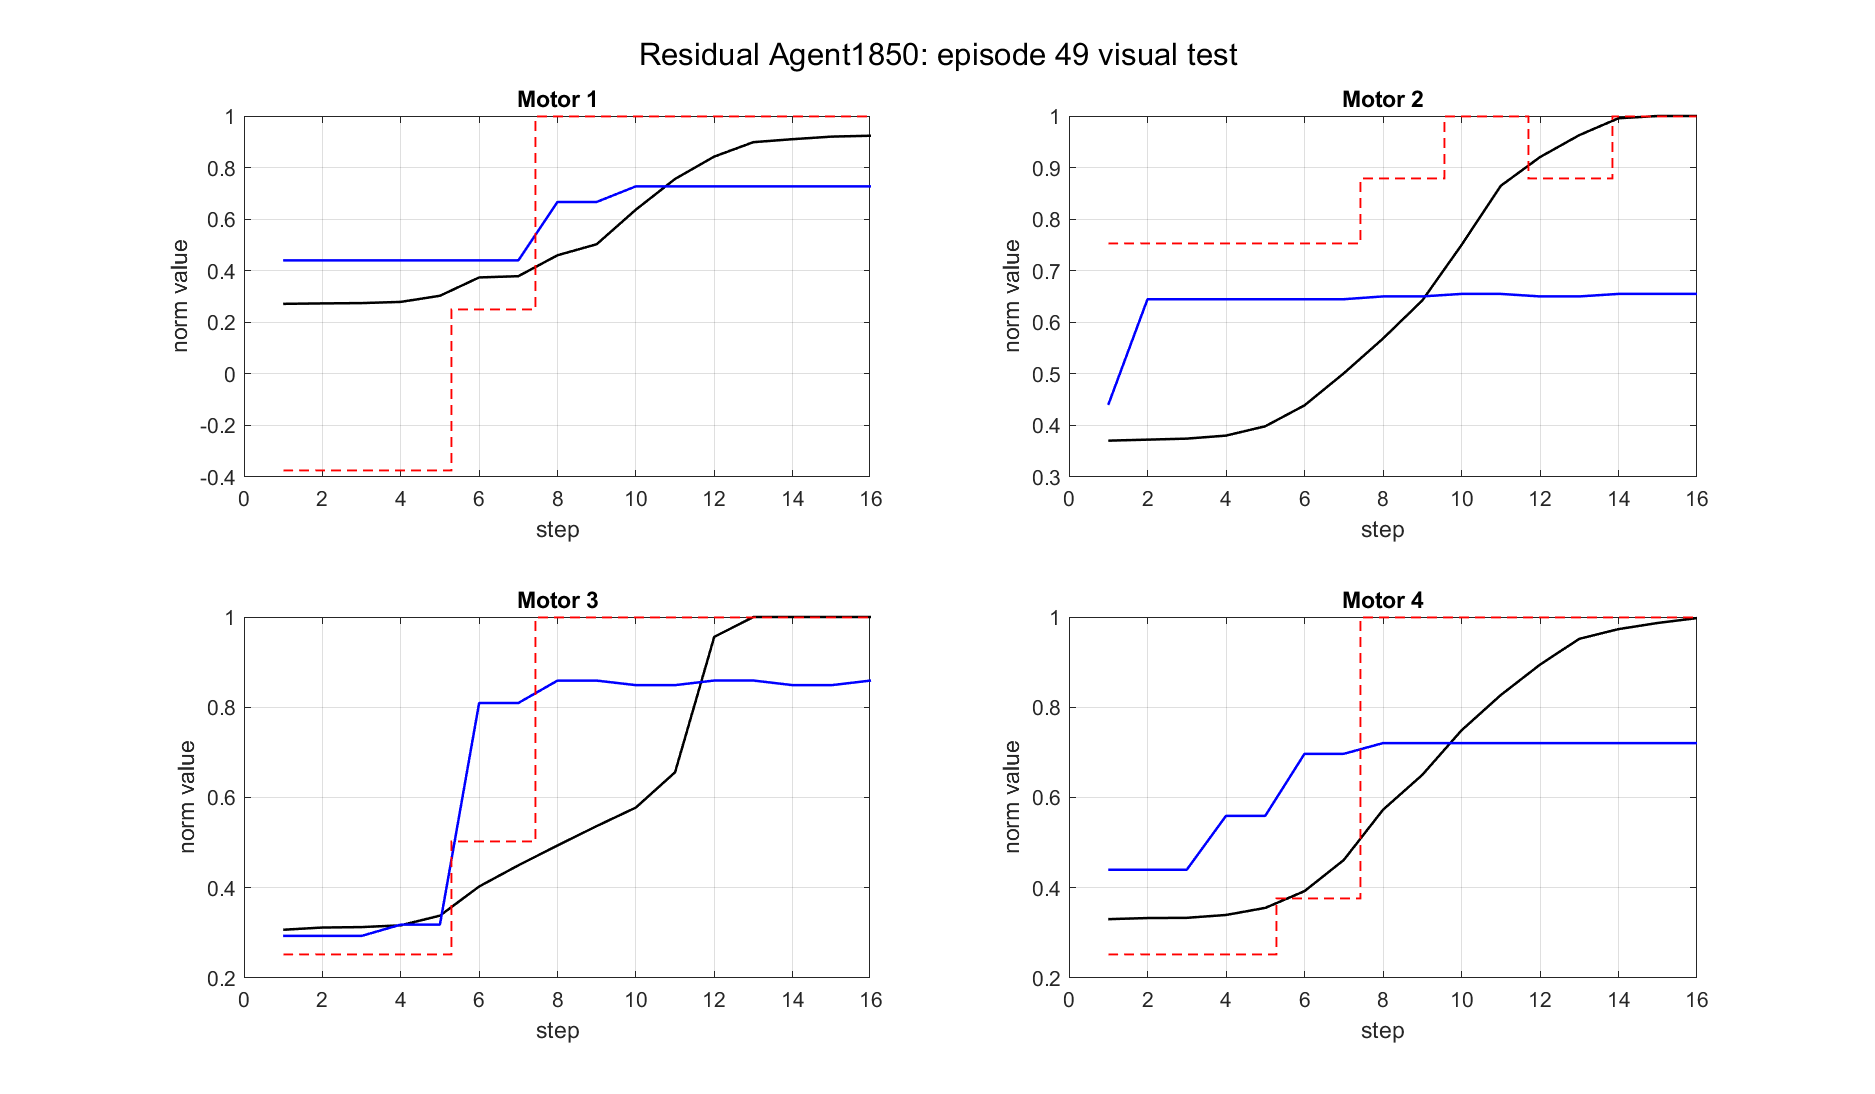
\includegraphics[width=\linewidth]{figures/residual_agent1850_episode49_20260326.png}
    \label{fig:res-test}
}
\caption{Residual pilot with $\alpha_{\mathrm{res}}=0.20$. The best checkpoint was not selected by final reward but by checkpoint audit and visual test. The representative test preserves tracking quality while reducing effective actuation intensity.}
\label{fig:residual-pilot}
\end{figure}

The best residual checkpoint was then extended with additional episodes to test whether simple continuation would keep improving the trade-off. It did not. The best checkpoint of the extended run degraded tracking and recovered much of the aggressiveness previously reduced. This result suggested that the relevant degree of freedom was not merely ``more episodes,'' but the amplitude of the residual correction itself.

The residual scale $\alpha_{\mathrm{res}}$ was then explored in two stages:
\begin{itemize}
    \item a coarse sweep: $\{0.10, 0.20, 0.30\}$;
    \item a fine sweep: $\{0.18, 0.20, 0.22, 0.25\}$.
\end{itemize}

These sweeps clarified the role of $\alpha_{\mathrm{res}}$:
\begin{itemize}
    \item small values under-corrected the frozen base;
    \item large values over-corrected and pushed the policy back toward high actuator usage;
    \item the best compromise remained centered at $\alpha_{\mathrm{res}}=0.20$.
\end{itemize}

\begin{figure}[!t]
\centering
\subfloat[Final metrics of the coarse and fine $\alpha_{\mathrm{res}}$ sweeps.]{
    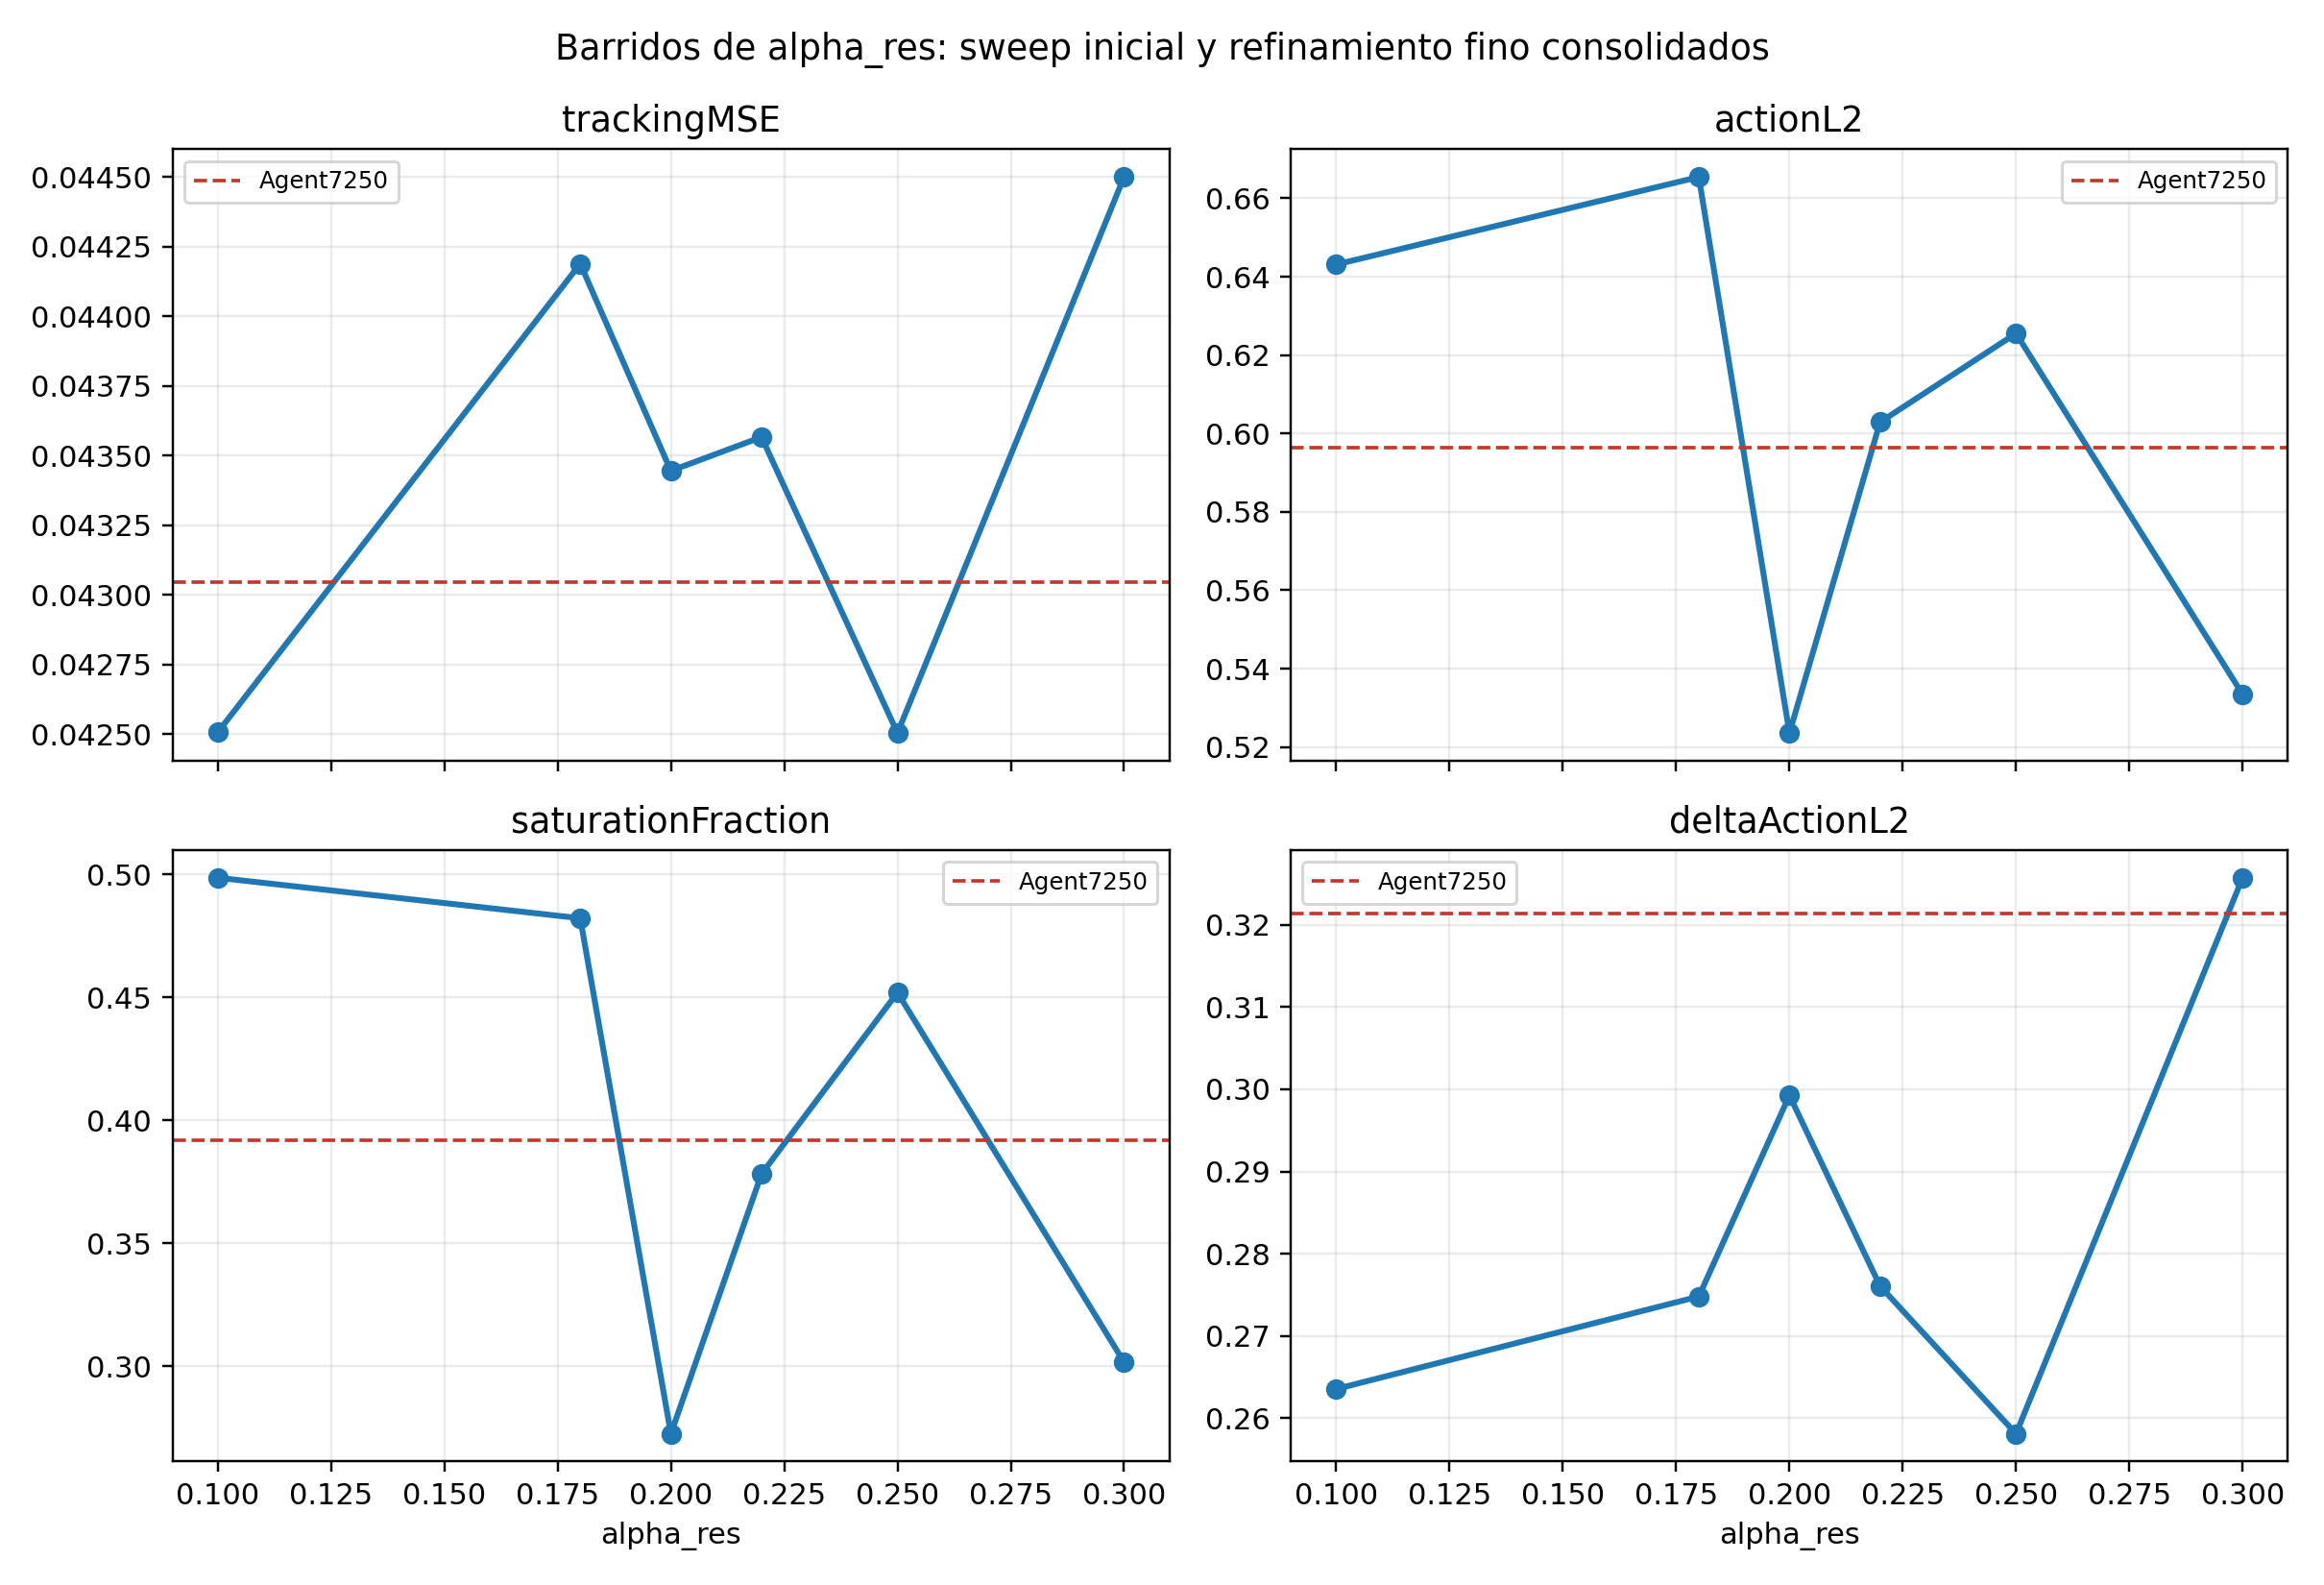
\includegraphics[width=\linewidth]{figures/residual_alpha_sweep_metrics_20260326.png}
    \label{fig:alpha-sweep}
}
\vspace{1mm}

\subfloat[Residual diagnostics versus $\alpha_{\mathrm{res}}$.]{
    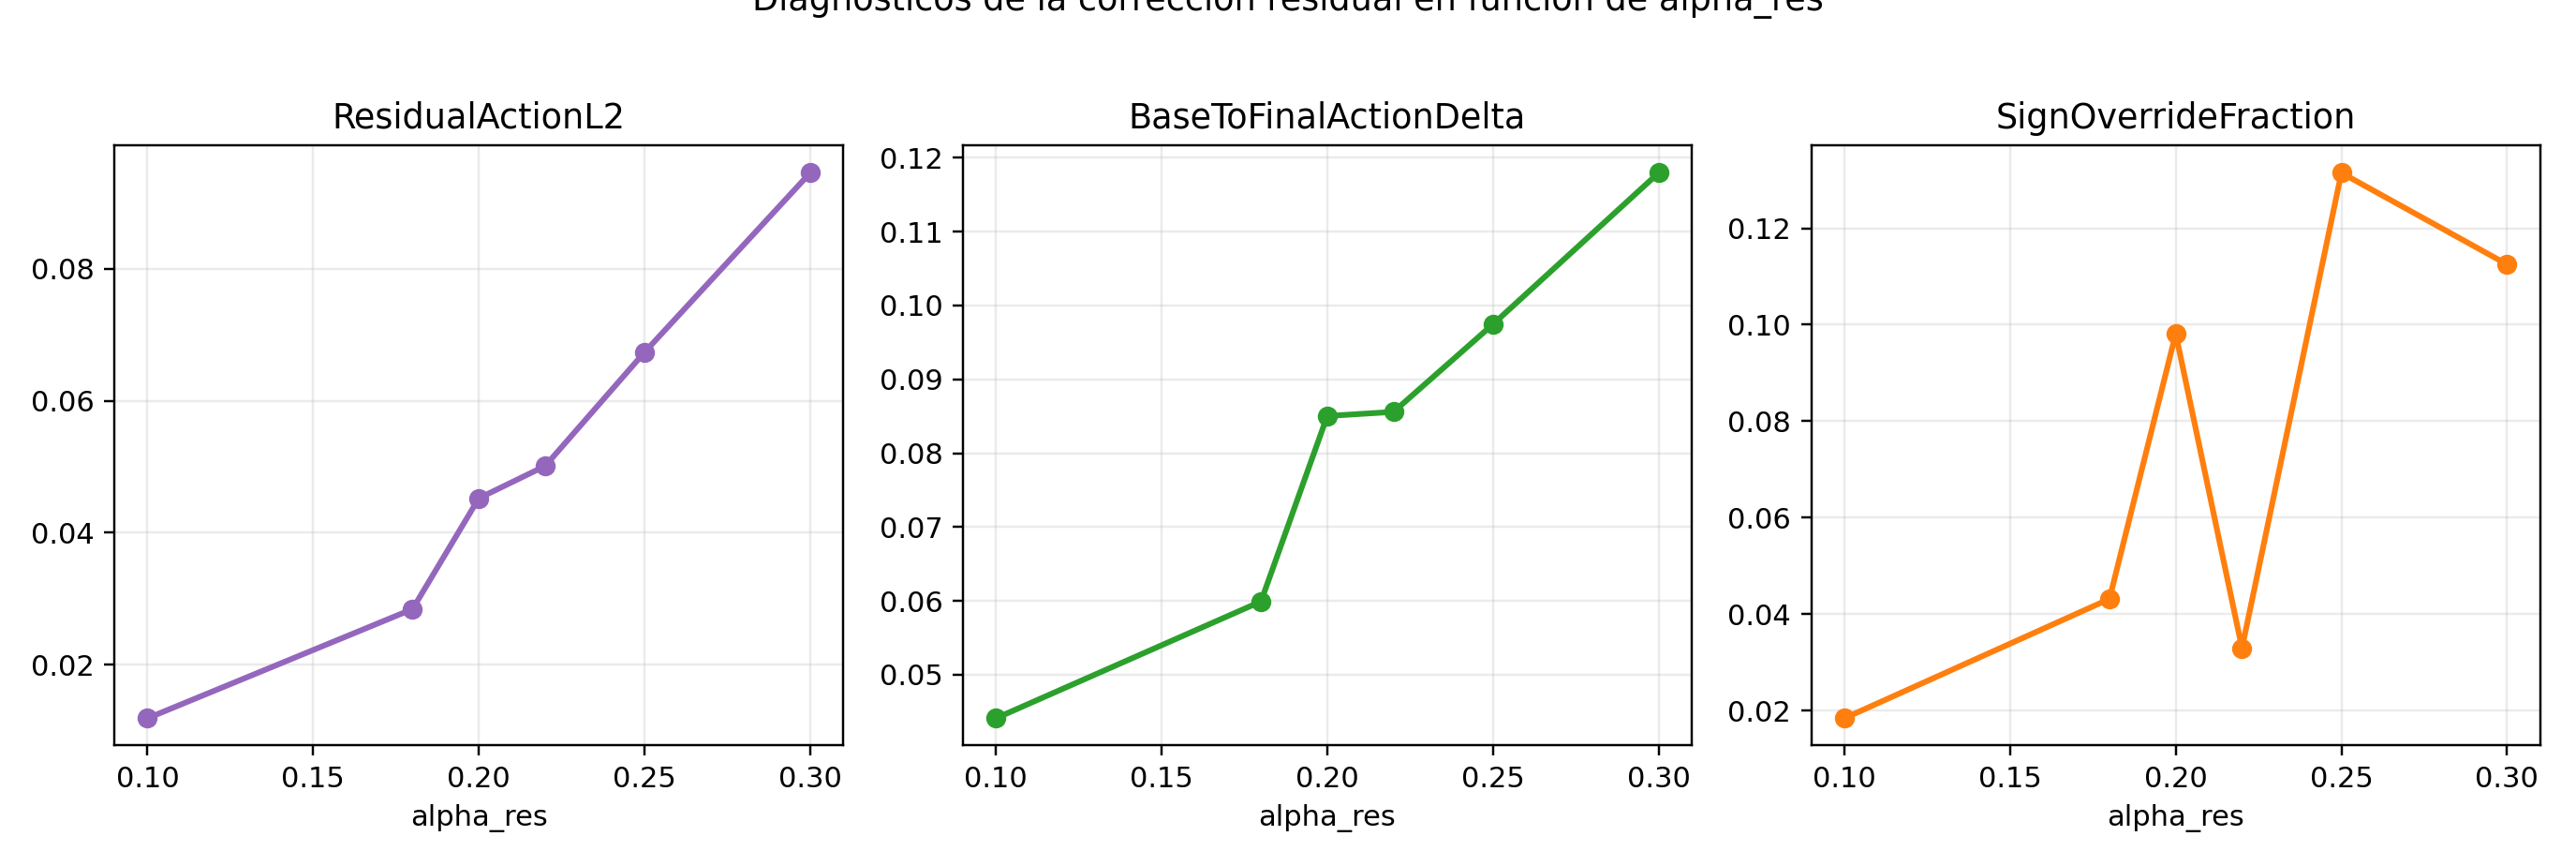
\includegraphics[width=\linewidth]{figures/residual_alpha_diagnostics_20260326.png}
    \label{fig:alpha-diagnostics}
}
\caption{Residual-scale analysis. The useful zone stayed around $\alpha_{\mathrm{res}}=0.20$. Larger values increased policy freedom but also actuator-edge behavior; smaller values failed to improve the base policy enough.}
\label{fig:alpha-analysis}
\end{figure}

\subsection{Reviewer-Facing Multi-seed Protocol}
The repository revision accompanying this paper adds a dedicated multi-seed launcher for the final residual method. The reproducibility protocol keeps the benchmark, residual scale, exploration parameters, and checkpoint-audit rule fixed, while varying only the random seed. The publication campaign uses seeds $\{11,22,33,44,55\}$, trains five independent residual pilots, selects the best checkpoint of each seed using the same tail-audit policy used throughout the project, and then evaluates each selected checkpoint with a final 50-simulation test.

This protocol is designed to produce per-seed final metrics for \texttt{trackingMSE}, \texttt{trackingMAE}, \texttt{actionL2}, \texttt{saturationFraction}, and \texttt{deltaActionL2}, together with aggregated \texttt{mean}~$\pm$~\texttt{std}, 95\% confidence intervals, and a count of how many seeds satisfy \texttt{ConditionA} or \texttt{ConditionB}. In other words, the repository now contains the exact instrumentation needed to answer the most important reviewer question: whether the residual improvement is stable beyond a single lucky training run.

\begin{table}[t]
\centering
\caption{Residual reproducibility summary for the five-seed campaign}
\label{tab:multiseed-results}
\footnotesize
\begin{tabularx}{\columnwidth}{L{2.15cm}Y}
\toprule
Statistic & Value \\
\midrule
Benchmark & \texttt{Agent7250} \\
Seeds & $\{11, 22, 33, 44, 55\}$ \\
Residual scale & $\alpha_{\mathrm{res}} = 0.20$ \\
Best accepted seed & Seed 22, \texttt{ConditionA} \\
Best tracking seed & Seed 55, rejected by effort/saturation \\ 
trackingMSE & $0.043785 \pm 0.001517$ \\
trackingMSE 95\% CI & $[0.041902,\; 0.045669]$ \\
trackingMAE & $0.161675 \pm 0.002406$ \\
actionL2 & $0.581119 \pm 0.069363$ \\
actionL2 95\% CI & $[0.495007,\; 0.667231]$ \\
saturationFraction & $0.336202 \pm 0.147114$ \\
saturationFraction 95\% CI & $[0.153566,\; 0.518839]$ \\
deltaActionL2 & $0.344544 \pm 0.036101$ \\
Acceptance counts & 1 \texttt{ConditionA}, 0 \texttt{ConditionB}, 4 rejected \\
\bottomrule
\end{tabularx}
\end{table}

\begin{figure}[t]
\centering
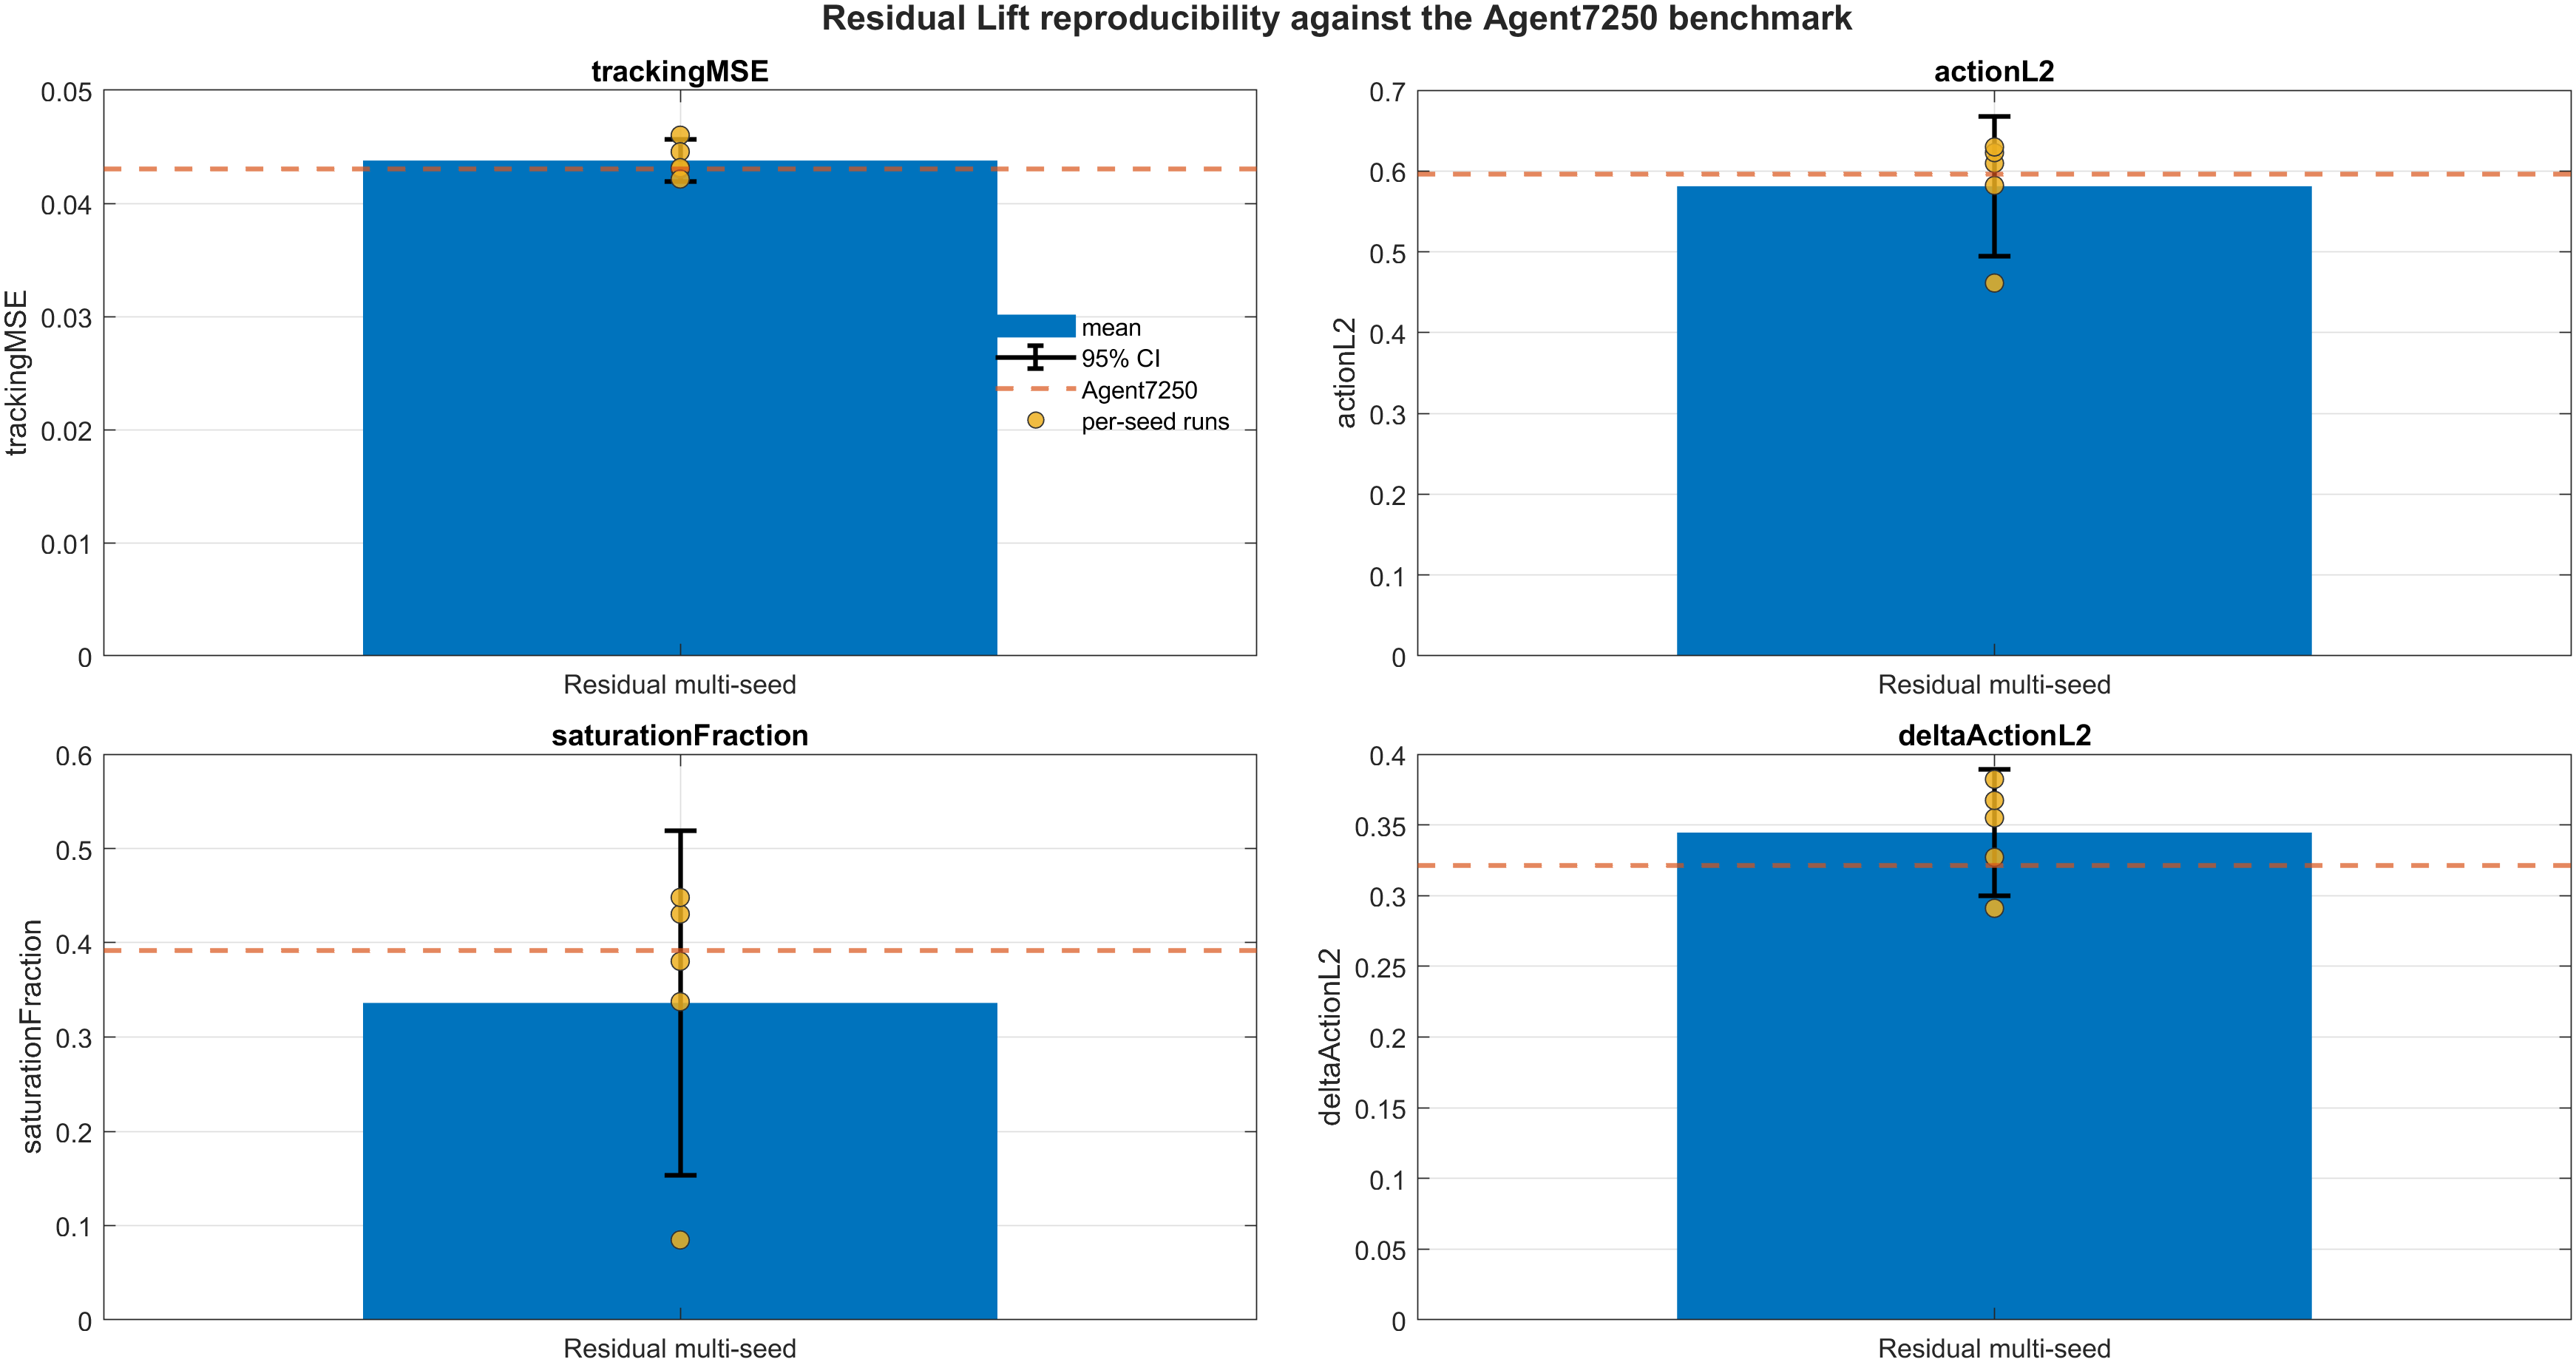
\includegraphics[width=\linewidth]{figures/residual_multiseed_summary_20260330.png}
\caption{Residual reproducibility across the five-seed campaign. The dashed line in each panel is the \texttt{Agent7250} benchmark. The bars show the multi-seed mean, the black error bars show the 95\% confidence interval, and the dots show the individual seeds. This figure makes the main reviewer-facing point explicit: the residual approach can produce a stronger single-run trade-off, but the variability across seeds remains non-negligible.}
\label{fig:multiseed}
\end{figure}

The completed five-seed campaign produced a stricter answer than the earlier three-seed version. Seed 22 was the only accepted run and satisfied \texttt{ConditionA} against the benchmark. Seeds 11, 33, 44, and 55 were rejected: seed 11 lost too much tracking, while seeds 33, 44, and 55 recovered too much aggressiveness despite competitive tracking values. Consequently, the repeated-run evidence does not support a claim of robust replacement of the benchmark. What it does support is narrower but still meaningful: residual fine-tuning remains the only intervention family in the repository that can occasionally outperform the benchmark trade-off, but its stability is not yet sufficient for a strong operational adoption claim.

\FloatBarrier

\section{Discussion}
Three findings emerge from the complete project timeline.

First, obtaining a defendable benchmark required more than choosing a strong RL algorithm. Reward clarity, temporal consistency, and simulator validity were prerequisites. Without those, numerical results were not scientifically meaningful.

Second, once a valid benchmark existed, several plausible interventions failed for understandable reasons. Lower-exploration continuation, saturation-aware shaping, offline warm-start, and action-interface warping each attacked one aspect of the problem, but none preserved the complete tracking--effort balance. This is precisely why a documented negative-result phase matters: it narrowed the design space and justified the residual hypothesis.

Third, the residual result is not just ``another checkpoint.'' The best single-run residual policy keeps the same observation, reward, quantized actuation, and benchmark reference, but improves the operational compromise with a modest correction term. Residual diagnostics support this interpretation: for the final $\alpha_{\mathrm{res}}=0.20$ model, the correction remained moderate, with residual-action energy around 0.0452, mean base-to-final action delta around 0.0850, and sign-override fraction around 0.0981. In other words, the residual branch improved the policy without replacing it. The five-seed campaign shows, however, that this positive mechanism is not yet a stable outcome of retraining.

\section{Limitations and External Validity}
This study remains simulation-based. Although the controller is built around prerecorded EMG and glove trajectories from multiple files in the repository, the present experiments do not constitute clinical validation, online subject-in-the-loop control, or hardware deployment. The current protocol also does not separate training and testing by held-out subject. Repetitions are sampled from a pooled prerecorded set, which is appropriate for controller development but does not establish inter-subject generalization.

The sample period of 0.2~s is part of the implemented control loop and is reported explicitly here because it materially shapes the practical horizon of the task. The reviewed myoelectric-control papers cited in this manuscript emphasize accuracy, task completion, or qualitative behavior more often than an explicit closed-loop cycle time, which limits direct latency comparison. Likewise, the benchmark values $\lambda_a = 0.01$, $\lambda_{\Delta a} = 0.05$, and $\gamma = 0.95$ are inherited from the validated benchmark configuration. They are justified operationally within this repository, but not presented as exhaustive hyperparameter optima. Future work should therefore include at least three extensions: subject-held-out evaluation, a dedicated latency analysis, and explicit ablations of $\gamma$ and reward weights.

Finally, even after extending the campaign to five seeds, the repeated-run evidence remains limited. The current manuscript can now report mean, standard deviation, and 95\% confidence intervals for the residual method, but only one of the five seeds satisfied the benchmark acceptance rule. This is a materially stronger position than a single-run claim, yet it still falls short of a fully stable statistical story. A larger seed study and, ideally, subject-held-out evaluation remain necessary before making stronger reproducibility claims.

\section{Conclusion}
This project now has a clear and reproducible methodological state. The valid post-fix baseline is \texttt{Agent7250}, obtained from the 8000-episode TD3 run. Multiple post-benchmark interventions were explored, but the only line that produced a strong single-run improvement was residual policy learning over the frozen benchmark. The best individual residual policy remains \texttt{Agent1850} with $\alpha_{\mathrm{res}}=0.20$, which satisfies \texttt{ConditionB} against the benchmark by preserving tracking while substantially reducing action energy and saturation.

The new five-seed campaign sharpens that conclusion. Residual fine-tuning is still the most promising intervention family in the repository, but the aggregate evidence does not justify presenting it as a robust replacement for the benchmark. The safer conclusion is therefore twofold: \texttt{Agent7250} remains the stable benchmark, and \texttt{Agent1850} remains the best single-run residual candidate. The broader lesson is methodological as much as algorithmic: for myoelectric prosthesis control under quantized actuation, the crucial gains came from establishing a valid baseline, applying a constrained residual correction, and then measuring how sensitive that correction is to repeated training. The revised repository now supports that fuller story with an explicit five-seed protocol, clearer dataset documentation, and a more honest statement of the limits of simulation-only evidence.

\clearpage
\section*{Acknowledgment}
The author thanks the Research Laboratory in Artificial Intelligence and Computer Vision ``Alan Turing'' for supporting this work and the iterative experimental process documented in the repository.

\bibliographystyle{IEEEtran}
\bibliography{references}

\end{document}
